

%% Mechanics Questions used on the
%% NYSED Physics Regents Examination
%%--------------------------------------------------

%% this section contains XX problems


%% Section June1986
%%--------------------
\newcommand{\nysedJuneNineteenEightySixQSeventyThree}{
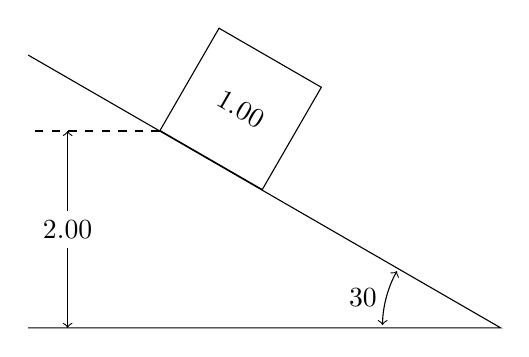
\begin{tikzpicture}
    %% ramp
    \draw (-6,0) -- (0,0) -- (150:{6/cos(30)});
    \draw[<->,shorten >=1pt,shorten <=1pt] (-1.5,0) arc(180:150:1.5)
        node[pos=0.5,anchor=east] {\ang{30}};
    %% object
    \node[draw,anchor=south,rotate=-30,minimum size=1.5cm] at (150:4.25) {\SI{1.00}{\kilo\gram}};
    \draw[dashed] (150:5) -- ++(180:{6-5*cos(30)});
    \draw[<->] (-5.5,0) -- (-5.5,{5*sin(30)})
        node[pos=0.5,anchor=center,fill=white] {\SI{2.00}{\meter}};
\end{tikzpicture}
}

\element{nysed}{
\begin{question}{June1986-Q73}
    The diagram represents a \SI{1.00}{\kilo\gram} object being held at rest on a frictionless incline.
    \begin{center}
        \nysedJuneNineteenEightySixQSeventyThree
    \end{center}
    The object is released and slides the length of the incline.
    When it reaches the bottom of the incline,
        the object's kinetic energy will be closest to:
    \begin{multicols}{2}
    \begin{choices}
      \correctchoice{\SI{19.8}{\joule}}
        \wrongchoice{\SI{2.00}{\joule}}
        \wrongchoice{\SI{9.81}{\joule}}
        \wrongchoice{\SI{4.00}{\joule}}
    \end{choices}
    \end{multicols}
\end{question}
}

\element{nysed}{
\begin{question}{June1986-Q74}
    The diagram represents a \SI{1.00}{\kilo\gram} object being held at rest on a frictionless incline.
    \begin{center}
        \nysedJuneNineteenEightySixQSeventyThree
    \end{center}
    If the angle between the incline and the horizontal surface is increased,
        the magnitude of the force needed to hold the object at rest on the inline will:
    \begin{choices}
        \wrongchoice{decrease}
      \correctchoice{increase}
        \wrongchoice{remain the same}
    \end{choices}
\end{question}
}

\element{nysed}{
\begin{question}{June1986-Q75}
    The diagram represents a \SI{1.00}{\kilo\gram} object being held at rest on a frictionless incline.
    \begin{center}
        \nysedJuneNineteenEightySixQSeventyThree
    \end{center}
    As the object slides down the incline,
        the sum of the gravitational potential energy and kinetic energy of the object will:
    \begin{choices}
        \wrongchoice{decrease}
        \wrongchoice{increase}
      \correctchoice{remain the same}
    \end{choices}
\end{question}
}


\endinput


